	\section{Domainmodel} 
		\subsection{Domain}
		
			\subsubsection{Verknüpfungen von Task-Vorlagen und Entscheidungs-Vorlagen}			
				Entscheidungs-Vorlagen werden Task-Vorlagen zugeordnet.
				Aus diesen TAsk-Vorlagen werden beim Export Tasks generiert.
				Task-Vorlagen sind generisch, da Änderungen auch alle verknüpften Entscheidungs-Vorlagen betreffen sollen.
				Aus diesem Grund werden Task-Vorlagen bei der Zuordnung verknüpft und nicht kopiert.
				
				\begin{figure}[H]
					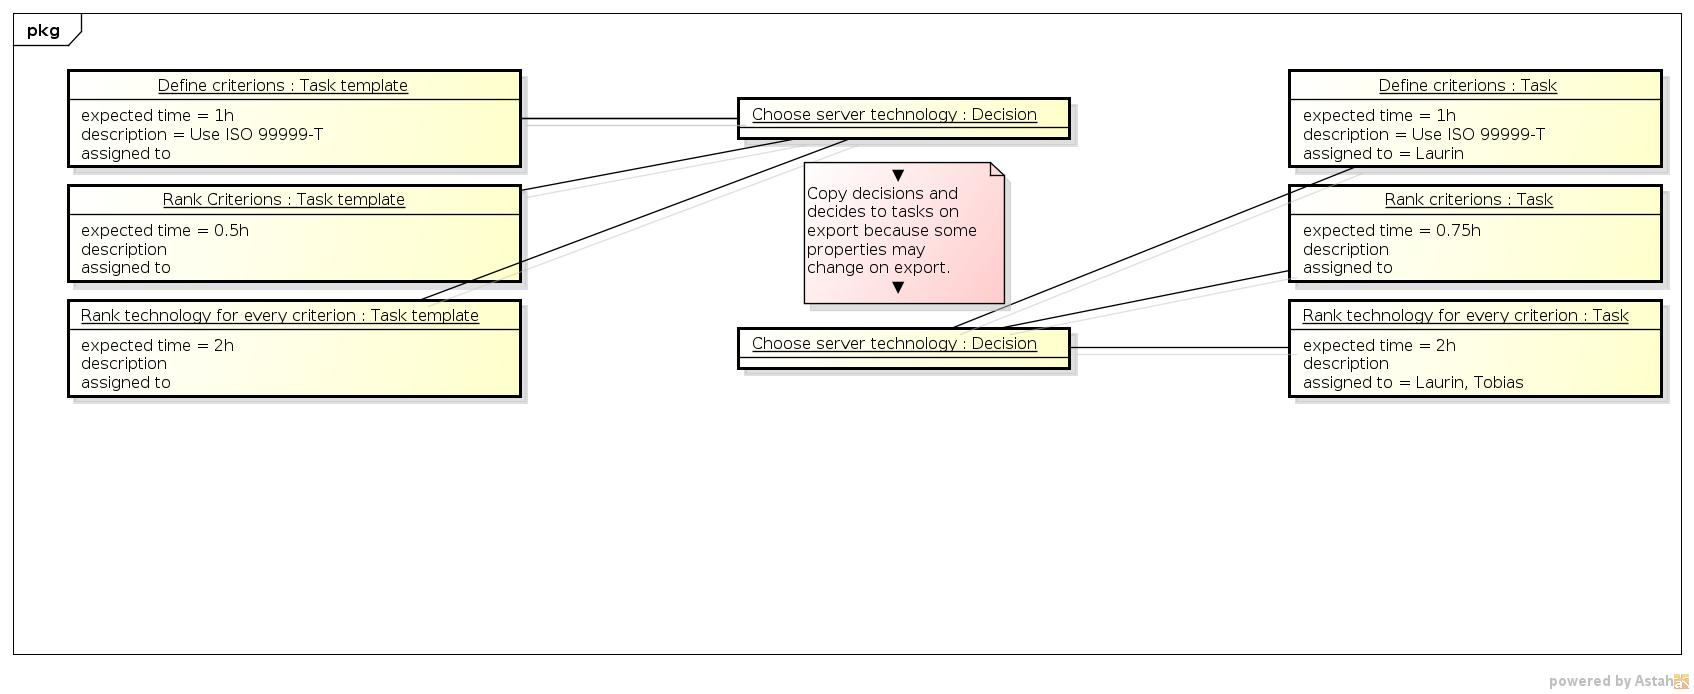
\includegraphics[width=\textwidth]{architecture/media/img/DecisionTaskRelation.jpg}
					\centering
					\caption{Exportieren von Entscheidungen}
					\label{fig:DecisionTaskRelation}
				\end{figure}
				
				Beim Exporten werden aus Task-Vorlagen (konkrete) Tasks.
				Auch Entscheidungen werden zu Tasks.
				Mit Entscheidungen verknüpfte Tasks werden dann zu Sub-Tasks.
				
				Benutzer wollen beim Export die von der Task-Vorlage vorgegebenen Werte möglicherweise anpassen, wie z.B. den erwarteten Aufwand für den Task.
				Daher ist es sinnvoll, die Eigenschaften der Task-Vorlagen in die (konkreten) Tasks zu kopieren, anstatt sie lediglich zu verknüpfen.
				Gleiches gilt für Entscheidungen. Würde jemand im CDAR diese verändern oder Löschen, so würde dies die History zerstören.
				
			
			\subsubsection{EEPPI Domain}
			
				
		
		\subsection{Communication}